\documentclass[aspectratio=169,11pt]{beamer}
\usepackage{amsmath,amssymb,booktabs,tikz,graphicx}
\usetikzlibrary{arrows.meta,positioning,fit,calc,shapes.geometric}

% ---------------------------------------------------------------- look
\definecolor{ink}{HTML}{1F2A44}
\definecolor{muted}{HTML}{5B6478}
\definecolor{sem}{HTML}{2A78D6}      % cross-encoder / semantic score
\definecolor{ctx}{HTML}{EB6834}      % GAT / contextual score
\definecolor{good}{HTML}{1BAF7A}
\definecolor{card}{HTML}{F1F4F9}
\definecolor{ctxcard}{HTML}{FDF0E9}
\definecolor{semcard}{HTML}{EAF2FC}

\usefonttheme{professionalfonts}
\setbeamertemplate{navigation symbols}{}
\setbeamercolor{normal text}{fg=ink,bg=white}
\setbeamercolor{frametitle}{fg=ink,bg=white}
\setbeamercolor{title}{fg=white}
\setbeamercolor{subtitle}{fg=white}
\setbeamercolor{structure}{fg=sem}
\setbeamercolor{itemize item}{fg=ctx}
\setbeamercolor{itemize subitem}{fg=muted}
\setbeamercolor{block title}{fg=white,bg=ink}
\setbeamercolor{block body}{bg=card}
\setbeamerfont{frametitle}{size=\LARGE,series=\bfseries}
\setbeamertemplate{itemize items}[circle]
\setbeamertemplate{frametitle}{\vspace*{0.35cm}\insertframetitle\par\vspace*{-0.15cm}}
\setbeamertemplate{footline}{%
  \hfill{\color{muted}\scriptsize\insertframenumber\,/\,\inserttotalframenumber}\hspace*{0.5cm}\vspace*{0.3cm}}
\setlength{\leftmargini}{1.1em}

\newcommand{\ssem}{s_{\mathrm{sem}}}
\newcommand{\sctx}{s_{\mathrm{ctx}}}
\newcommand{\src}[1]{\par\vfill{\color{muted}\scriptsize #1}}
\newcommand{\hl}[1]{{\color{ctx}\bfseries #1}}
\newcommand{\cardbox}[3][card]{%
  \begin{tikzpicture}\node[fill=#1,rounded corners=6pt,inner sep=8pt,text width=#2,align=left]{#3};\end{tikzpicture}}

% section divider: dark slide
\newcommand{\divider}[2]{%
{\setbeamercolor{background canvas}{bg=ink}\setbeamertemplate{footline}{}
\begin{frame}[plain]
  \vfill\begin{center}{\color{ctx}\Large\bfseries #1}\\[0.3cm]{\color{white}\Huge\bfseries #2}\end{center}\vfill
\end{frame}}}

\title{Alpha Follows the Hops}
\subtitle{Query Complexity and Score Fusion in Graph-Augmented Re-ranking}
\author{Tanish Verma \quad Narmety Vamshi \quad Pruthviraj Sharad Salunke}
\institute{Mehta Family School of Data Science \& Artificial Intelligence\\Indian Institute of Technology Roorkee}
\date{}

\begin{document}

% ================================================================ title
{\setbeamercolor{background canvas}{bg=ink}\setbeamertemplate{footline}{}
\begin{frame}[plain]
  \vspace*{0.6cm}
  {\color{ctx}\large\bfseries Relevant passage ranking}\\[0.25cm]
  {\color{white}\fontsize{34}{38}\selectfont\bfseries Alpha Follows the Hops}\\[0.3cm]
  {\color{white!85!ink}\Large Query Complexity and Score Fusion in Graph-Augmented Re-ranking}\\[1.1cm]
  {\color{white}\large Tanish Verma \quad Narmety Vamshi \quad Pruthviraj Sharad Salunke}\\[0.15cm]
  {\color{white!70!ink}Mehta Family School of Data Science \& Artificial Intelligence, IIT Roorkee}
  \vfill
  \begin{tikzpicture}[overlay,remember picture]
    \foreach \x/\c in {0/sem,0.9/ctx,1.8/good}{\fill[\c] ($(current page.south east)+(-2.6+\x,0.9)$) circle (0.22);}
    \draw[white!60!ink,line width=1.2pt] ($(current page.south east)+(-2.38,0.9)$)--++(0.46,0) ($(current page.south east)+(-1.48,0.9)$)--++(0.46,0);
  \end{tikzpicture}
\end{frame}}

% ================================================================ background
\divider{Part 1}{Background}

\begin{frame}{The task: rank passages for a query}
\begin{columns}[T]
\begin{column}{0.47\textwidth}
\begin{itemize}\setlength{\itemsep}{8pt}
  \item Input: a query $q$ and a pool of candidate passages $p_1,\dots,p_K$.
  \item Output: the passages ordered by relevance to $q$.
  \item A \hl{scoring function} gives each pair $(q,p_i)$ a score $s(q,p_i)$; the ranking sorts by it.
  \item Usual pipeline: a cheap retriever fills the pool (BM25, top-$K$), an expensive model \emph{re-ranks} it.
  \item Evaluated with nDCG@10 and MRR@10.
\end{itemize}
\end{column}
\begin{column}{0.5\textwidth}
\centering
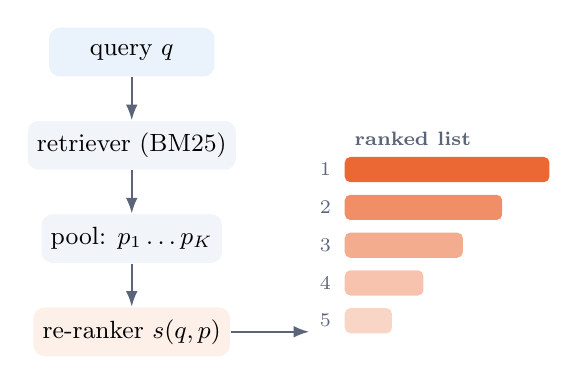
\begin{tikzpicture}[font=\small,
  box/.style={draw=none,fill=card,rounded corners=4pt,minimum height=0.62cm,minimum width=2.1cm},
  arr/.style={-{Latex[length=2mm]},thick,muted}]
  \node[box,fill=semcard] (q) {query $q$};
  \node[box,below=0.55cm of q] (ret) {retriever (BM25)};
  \node[box,below=0.55cm of ret] (pool) {pool: $p_1\dots p_K$};
  \node[box,fill=ctxcard,below=0.55cm of pool] (rr) {re-ranker $s(q,p)$};
  \draw[arr] (q)--(ret); \draw[arr] (ret)--(pool); \draw[arr] (pool)--(rr);
  \foreach \i/\w/\c in {0/2.6/ctx,1/2.0/ctx!75,2/1.5/ctx!55,3/1.0/ctx!40,4/0.6/ctx!28}{
    \fill[\c,rounded corners=2pt] ($(rr.east)+(1.45,1.9-\i*0.48)$) rectangle ++(\w,0.32);
    \node[font=\scriptsize,anchor=east,muted] at ($(rr.east)+(1.4,2.06-\i*0.48)$) {\pgfmathparse{int(\i+1)}\pgfmathresult};}
  \node[font=\scriptsize\bfseries,muted,anchor=west] at ($(rr.east)+(1.45,2.45)$) {ranked list};
  \draw[arr] (rr.east)--++(1.0,0);
\end{tikzpicture}
\end{column}
\end{columns}
\end{frame}

\begin{frame}{Scoring functions: one score per pair}
\centering
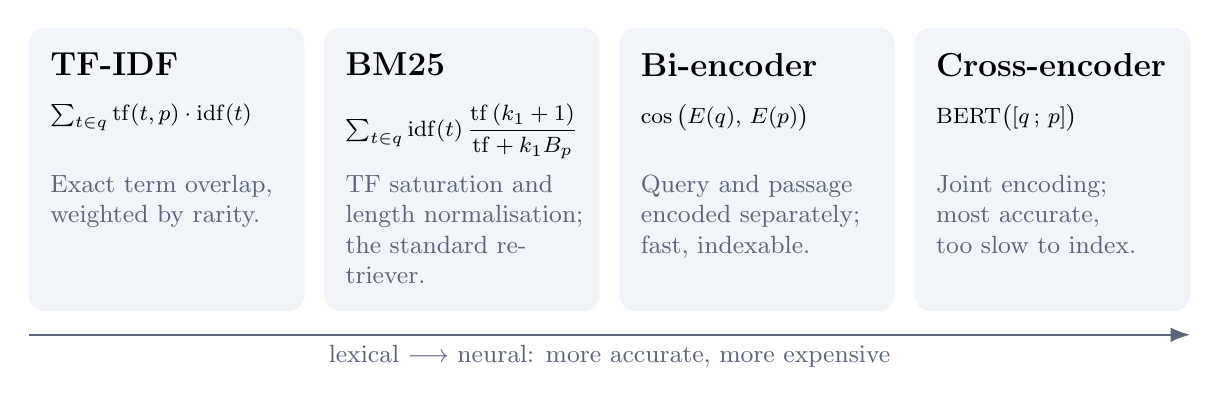
\begin{tikzpicture}[every node/.style={align=left,anchor=north west}]
  \foreach \x/\t/\f/\d in {
    0/TF-IDF/{$\sum_{t\in q}\mathrm{tf}(t,p)\cdot\mathrm{idf}(t)$}/{Exact term overlap,\\weighted by rarity.},
    3.75/BM25/{$\sum_{t\in q}\mathrm{idf}(t)\,\dfrac{\mathrm{tf}\,(k_1+1)}{\mathrm{tf}+k_1 B_p}$}/{TF saturation and\\length normalisation;\\the standard retriever.},
    7.5/Bi-encoder/{$\cos\big(E(q),\,E(p)\big)$}/{Query and passage\\encoded separately;\\fast, indexable.},
    11.25/Cross-encoder/{$\mathrm{BERT}\big([q\,;\,p]\big)$}/{Joint encoding;\\most accurate,\\too slow to index.}}{
    \fill[card,rounded corners=6pt] (\x,0) rectangle ++(3.5,-3.6);
    \node[font=\large\bfseries] at (\x+0.15,-0.2) {\t};
    \node[font=\footnotesize,text width=3.2cm] at (\x+0.15,-0.85) {\f};
    \node[font=\small,text width=3.2cm,muted] at (\x+0.15,-1.75) {\d};}
  \draw[-{Latex[length=2.5mm]},thick,muted] (0,-3.9)--node[below,font=\small]{lexical $\longrightarrow$ neural: more accurate, more expensive} (14.75,-3.9);
\end{tikzpicture}
\vspace{0.25cm}

\cardbox[ctxcard]{13.6cm}{All of them score each passage \textbf{on its own}: $s(q,p_i)$ never looks at the other candidates.}
\end{frame}

\begin{frame}{Where it breaks: multi-hop questions}
\begin{columns}[T]
\begin{column}{0.5\textwidth}
\textbf{Single-hop}: one passage answers the query.\\[0.3cm]
\textbf{Multi-hop}: the answer needs a \hl{chain} of passages.\\[0.4cm]
\begin{itemize}\setlength{\itemsep}{5pt}
  \item The second passage (about the director) shares almost no words with the query.
  \item A pointwise scorer ranks it low, although it is needed.
  \item Its relevance shows only \emph{through its link} to P1.
\end{itemize}
\end{column}
\begin{column}{0.47\textwidth}
\centering
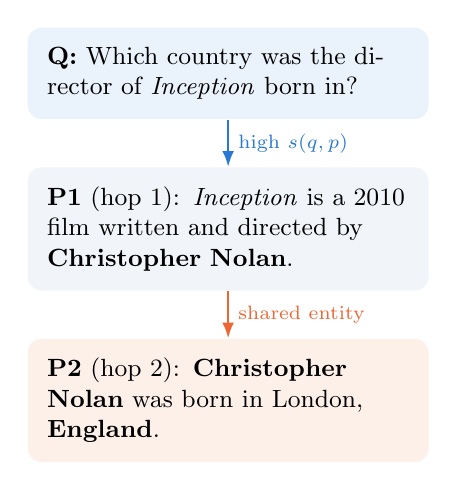
\begin{tikzpicture}[font=\small,
  pas/.style={fill=card,rounded corners=5pt,text width=4.6cm,inner sep=7pt,align=left}]
  \node[pas,fill=semcard] (q) {\textbf{Q:} Which country was the director of \emph{Inception} born in?};
  \node[pas,below=0.6cm of q] (p1) {\textbf{P1} (hop 1): \emph{Inception} is a 2010 film written and directed by \textbf{Christopher Nolan}.};
  \node[pas,below=0.6cm of p1,fill=ctxcard] (p2) {\textbf{P2} (hop 2): \textbf{Christopher Nolan} was born in London, \textbf{England}.};
  \draw[-{Latex[length=2mm]},thick,sem] (q)--node[right,font=\scriptsize]{high $s(q,p)$}(p1);
  \draw[-{Latex[length=2mm]},thick,ctx] (p1)--node[right,font=\scriptsize]{shared entity}(p2);
\end{tikzpicture}\\[0.1cm]
{\scriptsize\color{muted}Illustrative example.}
\end{column}
\end{columns}
\end{frame}

\begin{frame}{GAR: Graph-based Adaptive Re-ranking}
\begin{columns}[T]
\begin{column}{0.56\textwidth}
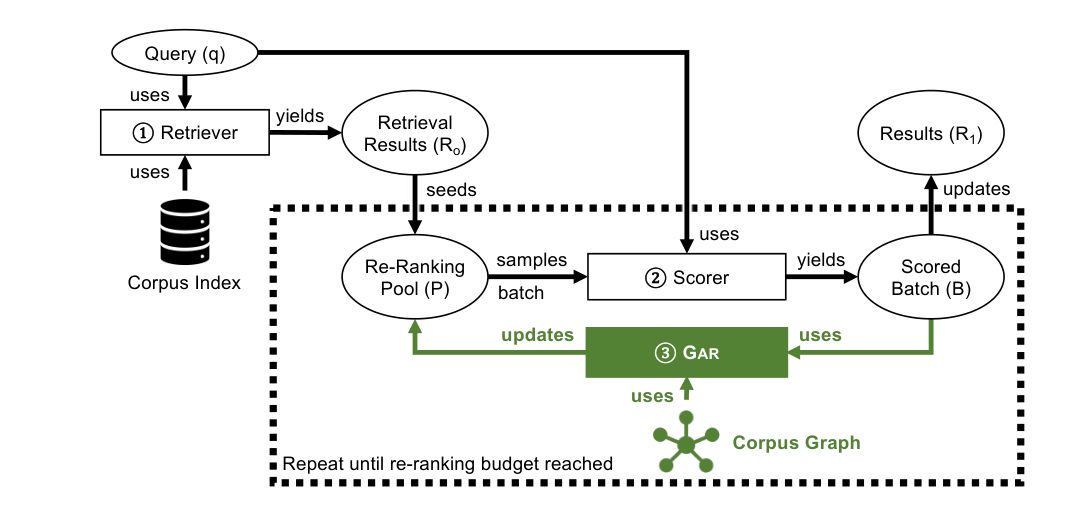
\includegraphics[width=\linewidth]{img/gar_fig1.png}\\[0.1cm]
{\scriptsize\color{muted}Figure 1 of MacAvaney et al.\ (CIKM 2022).}
\end{column}
\begin{column}{0.41\textwidth}
\begin{itemize}\setlength{\itemsep}{6pt}
  \item \textbf{Clustering hypothesis}: passages close to a relevant passage tend to be relevant too.
  \item Offline: a \hl{corpus graph}, each passage linked to its $k$ most similar passages.
  \item Online: after each scored batch, the \emph{neighbours} of the top passages join the pool.
  \item Fixes the recall limit of the first-stage pool; the scorer itself stays pointwise.
\end{itemize}
\end{column}
\end{columns}
\end{frame}

\begin{frame}{GAR: the re-ranking loop}
\begin{columns}[c]
\begin{column}{0.48\textwidth}
\centering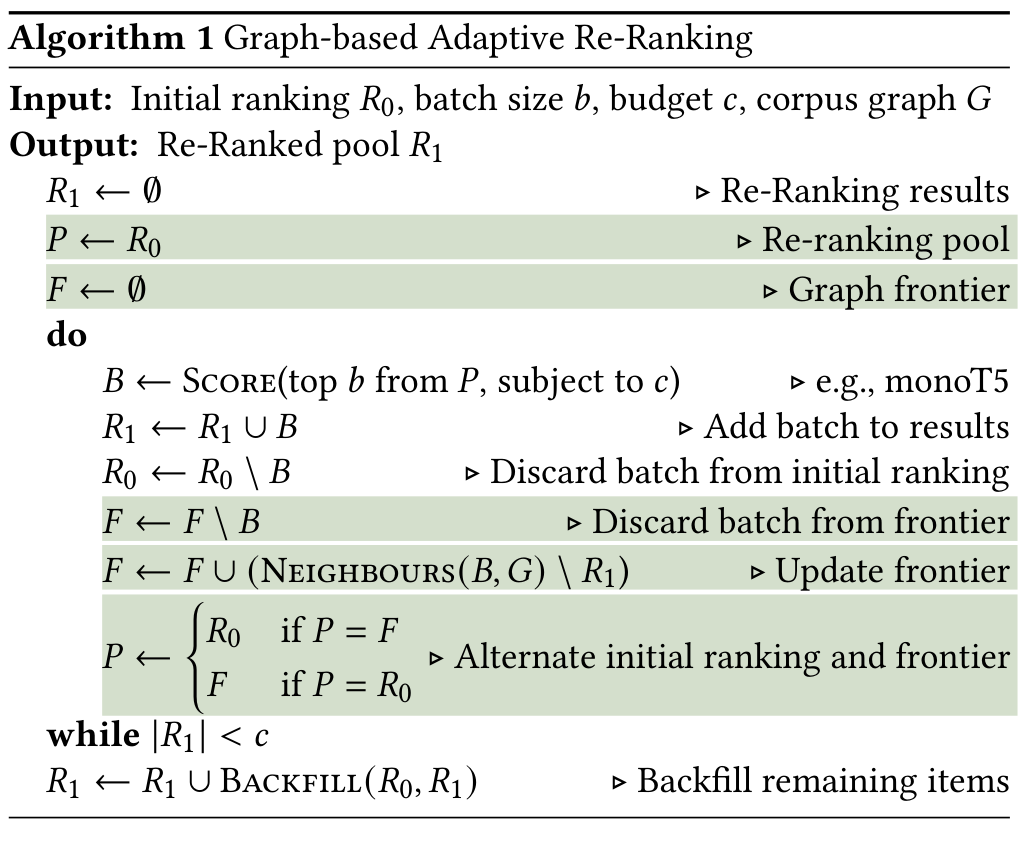
\includegraphics[width=0.93\linewidth]{img/gar_alg1.png}\\[0.05cm]
{\scriptsize\color{muted}Algorithm 1 of MacAvaney et al.\ (CIKM 2022).}
\end{column}
\begin{column}{0.48\textwidth}
\begin{itemize}\setlength{\itemsep}{8pt}
  \item Alternates between the initial ranking $R_0$ and the \emph{graph frontier} $F$.
  \item Up to +8\% nDCG for BM25 $\gg$ monoT5 on MS MARCO.
  \item The graph decides \hl{which} passages get scored, not \hl{how} they are scored.
\end{itemize}
\vspace{0.3cm}
\cardbox[semcard]{6.2cm}{\small\textbf{Next step:} let the graph change the \emph{score} itself, so a passage is judged together with its neighbours $\Rightarrow$ ReGAT-BERT.}
\end{column}
\end{columns}
\end{frame}

\begin{frame}{ReGAT-BERT: the idea}
\begin{columns}[T]
\begin{column}{0.49\textwidth}
\cardbox[semcard]{6.3cm}{{\color{sem}\large\bfseries Semantic score $\ssem$}\\[0.15cm]
\small A BERT cross-encoder reads $(q,p)$ jointly.\\Strong on \emph{direct} matches.}
\vspace{0.3cm}

\cardbox[ctxcard]{6.3cm}{{\color{ctx}\large\bfseries Contextual score $\sctx$}\\[0.15cm]
\small Passages form a graph; a Graph Attention Network refines each passage embedding with its neighbours.\\Scores the passage \emph{in context}.}
\end{column}
\begin{column}{0.47\textwidth}
\begin{itemize}\setlength{\itemsep}{8pt}
  \item Two complementary views of relevance.
  \item Final score = a weighted sum of the two:
  \[\mathrm{score}(q,p)=\alpha\,\ssem+\beta\,\sctx\]
  \item $\alpha,\beta$ are learned \textbf{once}, then the \hl{same weights apply to every query}.
\end{itemize}
\end{column}
\end{columns}
\end{frame}

\begin{frame}{ReGAT-BERT architecture}
\centering\vspace{0.4cm}
\resizebox{\textwidth}{!}{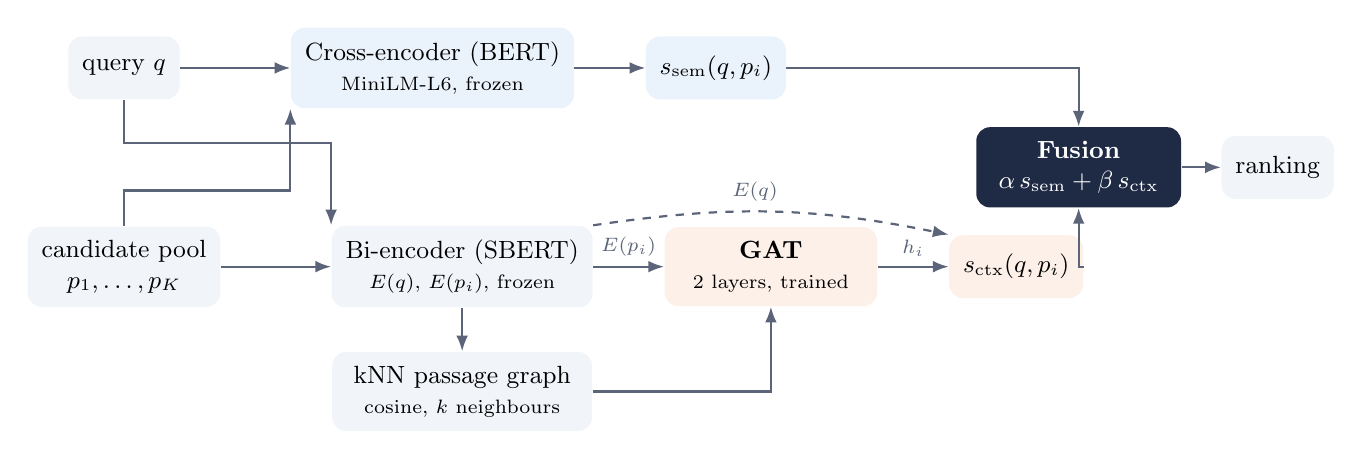
\begin{tikzpicture}[font=\small,
  blk/.style={rounded corners=5pt,minimum height=0.8cm,inner sep=5pt,align=center},
  arr/.style={-{Latex[length=2mm]},thick,muted}]
  \node[blk,fill=card] (q) {query $q$};
  \node[blk,fill=card,below=1.6cm of q] (p) {candidate pool\\$p_1,\dots,p_K$};
  % semantic branch
  \node[blk,fill=semcard,right=1.4cm of q,minimum width=3.3cm] (ce) {Cross-encoder (BERT)\\{\scriptsize MiniLM-L6, frozen}};
  \node[blk,fill=semcard,right=0.9cm of ce] (ss) {$\ssem(q,p_i)$};
  % context branch
  \node[blk,fill=card,right=1.4cm of p,minimum width=3.3cm] (be) {Bi-encoder (SBERT)\\{\scriptsize $E(q)$, $E(p_i)$, frozen}};
  \node[blk,fill=card,below=0.55cm of be,minimum width=3.3cm] (g) {kNN passage graph\\{\scriptsize cosine, $k$ neighbours}};
  \node[blk,fill=ctxcard,right=0.9cm of be,minimum width=2.7cm] (gat) {\textbf{GAT}\\{\scriptsize 2 layers, trained}};
  \node[blk,fill=ctxcard,right=0.9cm of gat] (sc) {$\sctx(q,p_i)$};
  % fusion
  \node[blk,fill=ink,text=white,minimum width=2.6cm] (fu) at ($(ss)!0.5!(sc)+(2.7,0)$) {\textbf{Fusion}\\$\alpha\,\ssem+\beta\,\sctx$};
  \node[blk,fill=card,right=0.5cm of fu] (r) {ranking};
  \draw[arr] (q)--(ce); \draw[arr] (q.south)--++(0,-0.55)-|(be.north west);
  \draw[arr] (p.north)--++(0,0.45)-|(ce.south west);
  \draw[arr] (p)--(be); \draw[arr] (be)--(g); \draw[arr] (be)--node[above,font=\scriptsize]{$E(p_i)$}(gat);
  \draw[arr] (g.east)-|(gat.south);
  \draw[arr] (ce)--(ss); \draw[arr] (gat)--node[above,font=\scriptsize]{$h_i$}(sc);
  \draw[arr] (ss.east)-|(fu.north); \draw[arr] (sc.east)-|(fu.south); \draw[arr] (fu)--(r);
  \draw[arr,dashed] (be.north east)to[bend left=10]node[pos=0.45,above,font=\scriptsize]{$E(q)$}(sc.north west);
\end{tikzpicture}}
\src{Our diagram of the pipeline as reproduced in this project (models as used in our experiments).}
\end{frame}

\begin{frame}{Inside the GAT: attention over neighbours}
\begin{columns}[T]
\begin{column}{0.52\textwidth}
\textbf{Graph}: node $i$ = passage $p_i$ with feature $x_i=E(p_i)$; edges to its $k$ nearest pool neighbours (cosine $\ge 0.3$) and a self-loop.\\[0.3cm]
\textbf{Attention} (GATv2, per head):
\[e_{ij}=\mathbf a^{\!\top}\,\mathrm{LeakyReLU}\big(\mathbf W[x_i\,\|\,x_j]\big)\]
\[\alpha_{ij}=\frac{\exp(e_{ij})}{\sum_{k\in\mathcal N(i)}\exp(e_{ik})},\qquad
x_i'=\sum_{j\in\mathcal N(i)}\alpha_{ij}\,\mathbf W x_j\]
\textbf{Two layers}: 4 heads (concat, hidden 128) $\to$ ELU $\to$ 1 head back to dimension $d$.
\end{column}
\begin{column}{0.44\textwidth}
\centering
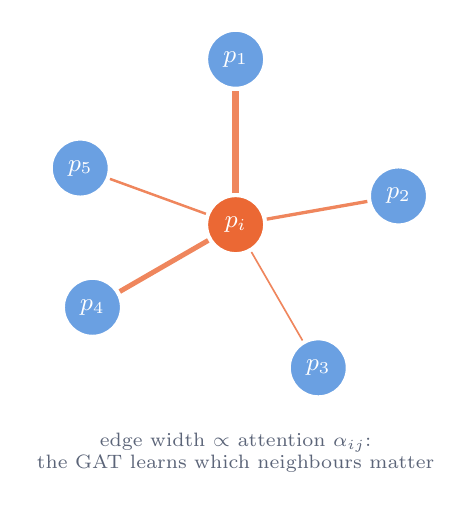
\begin{tikzpicture}[font=\small,
  n/.style={circle,draw=white,line width=1.5pt,minimum size=0.75cm,inner sep=0pt}]
  \node[n,fill=ctx,text=white] (i) at (0,0) {$p_i$};
  \foreach \a/\l/\w in {90/p_1/2.4,10/p_2/1.2,-60/p_3/0.6,-150/p_4/1.8,160/p_5/0.9}{
    \node[n,fill=sem!70,text=white] (\l) at (\a:2.1) {$\l$};
    \draw[ctx!80,line width=\w pt] (i)--(\l);}
  \node[font=\scriptsize,muted,align=center] at (0,-2.9) {edge width $\propto$ attention $\alpha_{ij}$:\\the GAT learns which neighbours matter};
\end{tikzpicture}
\end{column}
\end{columns}
\end{frame}

\begin{frame}{The contextual score: maths}
\begin{columns}[T]
\begin{column}{0.53\textwidth}
\textbf{1. Refine} each passage with its neighbourhood (residual, so it starts at the bi-encoder embedding):
\[h_i=\frac{\mathrm{LN}\big(x_i+\mathrm{GAT}(X,A)_i\big)}{\big\|\mathrm{LN}\big(x_i+\mathrm{GAT}(X,A)_i\big)\big\|}\]
\textbf{2. Score} against the query vector, which lives in the same space ($h_i\in\mathbb R^d$, $E(q)\in\mathbb R^d$):
\[\sctx(q,p_i)=E(q)^{\!\top}h_i=\cos\big(E(q),h_i\big)\]
\end{column}
\begin{column}{0.44\textwidth}
\textbf{3. Train} the GAT once (encoders frozen) with InfoNCE over the pool:
\[\mathcal L_{\mathrm{GAT}}=-\log\frac{\sum_{p^+}\exp(\sctx(q,p^+)/\tau)}{\sum_{j=1}^{K}\exp(\sctx(q,p_j)/\tau)}\]
{\small $\tau=0.05$; positives = gold passages.}\\[0.4cm]
\cardbox[ctxcard]{5.6cm}{\small Same query vector, but a passage's vector now carries information from the passages it is linked to, e.g.\ the bridge entity of a 2-hop chain.}
\end{column}
\end{columns}
\end{frame}

\begin{frame}{ReGAT-BERT fusion strategy}
\begin{columns}[c]
\begin{column}{0.55\textwidth}
\[\mathrm{score}(q,p)=\alpha\cdot\ssem(q,p)+\beta\cdot\sctx(q,p)\]
\begin{itemize}\setlength{\itemsep}{8pt}
  \item $\alpha,\beta$: two free scalars, learned with a pointwise BCE loss on relevance labels.
  \item Raw scores are fused as they are: the cross-encoder logit and the cosine live on \textbf{different scales}.
  \item One pair $(\alpha,\beta)$ for \hl{all queries}: an easy keyword query and a 4-hop question get the same mix.
\end{itemize}
\end{column}
\begin{column}{0.4\textwidth}
\centering
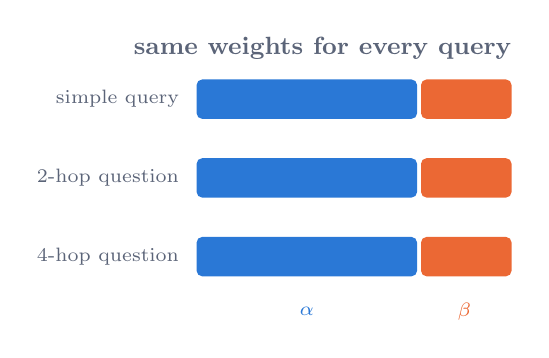
\begin{tikzpicture}
  \node[font=\small\bfseries,muted] at (1.6,3.3) {same weights for every query};
  \foreach \y/\l in {2.4/{simple query},1.4/{2-hop question},0.4/{4-hop question}}{
    \fill[sem,rounded corners=2pt] (0,\y) rectangle (2.8,\y+0.5);
    \fill[ctx,rounded corners=2pt] (2.85,\y) rectangle (4,\y+0.5);
    \node[font=\scriptsize,anchor=east,muted] at (-0.1,\y+0.25) {\l};}
  \node[font=\scriptsize,sem] at (1.4,-0.05) {$\alpha$};
  \node[font=\scriptsize,ctx] at (3.4,-0.05) {$\beta$};
\end{tikzpicture}
\end{column}
\end{columns}
\end{frame}

% ================================================================ our work
\divider{Part 2}{Our study}

\begin{frame}{Problem statement}
\cardbox[card]{13.6cm}{\large Should the weight between the semantic and the contextual score be \hl{the same for every query}, or should it depend on the query and its passages?}
\vspace{0.45cm}

\begin{columns}[T]
\begin{column}{0.47\textwidth}
\cardbox[semcard]{6.1cm}{{\color{sem}\bfseries Simple / single-hop queries}\\[0.1cm]
\small One passage answers it; the cross-encoder sees everything it needs.\\[0.1cm]
\textbf{Expect $\alpha>0.5$} (trust $\ssem$).}
\end{column}
\begin{column}{0.47\textwidth}
\cardbox[ctxcard]{6.1cm}{{\color{ctx}\bfseries Complex / multi-hop queries}\\[0.1cm]
\small Evidence is spread over linked passages; only the graph sees the links.\\[0.1cm]
\textbf{Expect $\alpha<0.5$} (trust $\sctx$).}
\end{column}
\end{columns}
\vspace{0.4cm}

{\bfseries Hypothesis:} $\alpha$ should \emph{fall as the number of hops rises}, so a query-dependent $\alpha(\cdot)$ should beat a single fixed $\alpha$.
\end{frame}

\begin{frame}{Our score and the normalisers}
\[\mathrm{score}(q,p_i)=\alpha\cdot\tilde s_{\mathrm{sem}}(q,p_i)+(1-\alpha)\cdot\tilde s_{\mathrm{ctx}}(q,p_i),\qquad \alpha\in(0,1)\]
{\small $\tilde s$ = score normalised \emph{within each query's pool}, so $\alpha$ is a true mixing weight. $\alpha=1$: cross-encoder only; $\alpha=0$: GAT only.}\\[0.25cm]
\centering
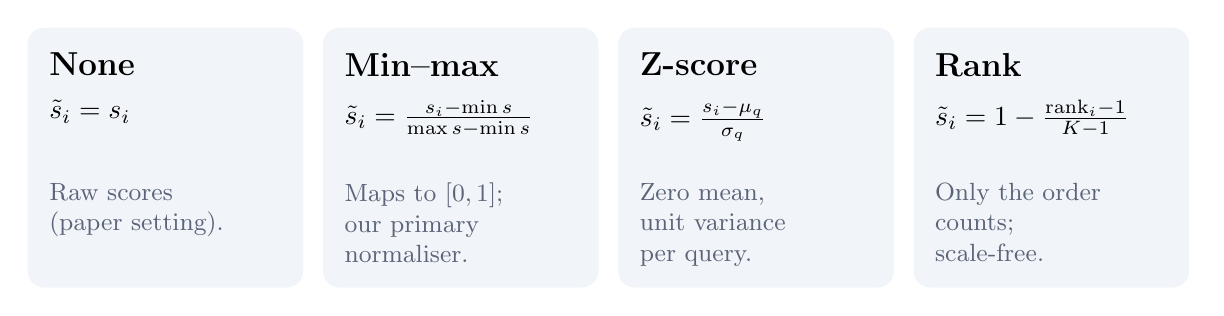
\begin{tikzpicture}[every node/.style={align=left,anchor=north west}]
  \foreach \x/\t/\f/\d in {
    0/None/{$\tilde s_i=s_i$}/{Raw scores\\(paper setting).},
    3.75/Min--max/{$\tilde s_i=\frac{s_i-\min s}{\max s-\min s}$}/{Maps to $[0,1]$;\\our primary\\normaliser.},
    7.5/Z-score/{$\tilde s_i=\frac{s_i-\mu_q}{\sigma_q}$}/{Zero mean,\\unit variance\\per query.},
    11.25/Rank/{$\tilde s_i=1-\frac{\mathrm{rank}_i-1}{K-1}$}/{Only the order\\counts;\\scale-free.}}{
    \fill[card,rounded corners=6pt] (\x,0) rectangle ++(3.5,-3.3);
    \node[font=\large\bfseries] at (\x+0.15,-0.2) {\t};
    \node[font=\normalsize,text width=3.2cm] at (\x+0.15,-0.8) {\f};
    \node[font=\small,text width=3.2cm,muted] at (\x+0.15,-1.85) {\d};}
\end{tikzpicture}
\end{frame}

\begin{frame}{Modelling the dependency of $\alpha$}
\begin{columns}[T]
\begin{column}{0.5\textwidth}
\textbf{Gate}: a small MLP whose \hl{input} decides what $\alpha$ may depend on:
\[\alpha(x)=\epsilon+(1-2\epsilon)\,\sigma\big(\mathbf w_2^{\top}\mathrm{ReLU}(\mathbf W_1x+\mathbf b_1)+b_2\big)\]
\renewcommand{\arraystretch}{1.25}
{\small
\begin{tabular}{@{}ll@{}}
\toprule
Gate & input $x$\\
\midrule
fixed & none: one learned scalar\\
\textbf{Q} & query embedding $E(q)\in\mathbb R^{384}$\\
\textbf{S} & 12 score statistics $f(\ssem,\sctx)$\\
\textbf{QS} & $[E(q)\,\|\,f]$\\
\textbf{QS+C} & $[E(q)\,\|\,f\,\|\,$len, \#entities$]$\\
\bottomrule
\end{tabular}}
\end{column}
\begin{column}{0.46\textwidth}
{\small\textbf{S features} (per query, from raw scores, never labels): for each of $\ssem$, $\sctx$: mean, std, top-1, top-1$-$top-2 gap, softmax entropy; plus Spearman$(\ssem,\sctx)$ and top-10 overlap.\\[0.25cm]
\textbf{Training} (CE and GAT frozen):
\[\mathcal L=-\log\!\sum_{p^+}\mathrm{softmax}_i\!\Big(\tfrac{\mathrm{score}_i}{T}\Big)+\lambda\,(\alpha-\alpha_0)^2\]
$b_2$ starts at $\mathrm{logit}(\alpha_0)$ ($\alpha_0$ = best fixed $\alpha$ on val): every gate starts as the fixed baseline. $\lambda=0.01$, 5 seeds.}
\end{column}
\end{columns}
\end{frame}

\begin{frame}{Datasets: from single-hop to multi-hop}
\centering
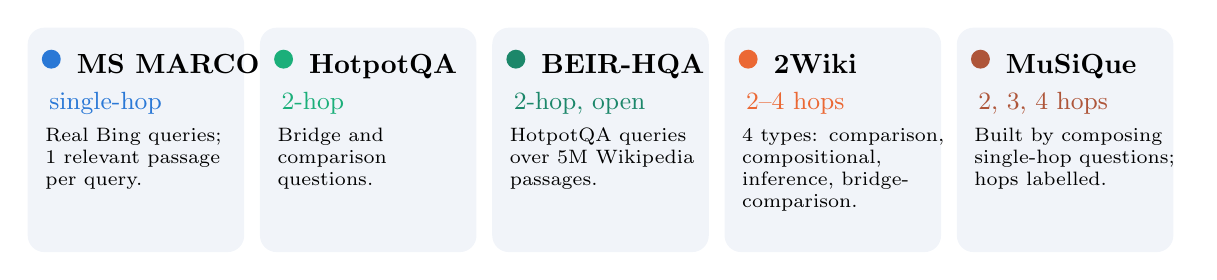
\begin{tikzpicture}[every node/.style={align=left,anchor=north west}]
  \foreach \x/\c/\t/\h/\d in {
    0/sem/MS MARCO/single-hop/{Real Bing queries;\\1 relevant passage\\per query.},
    2.95/good/HotpotQA/2-hop/{Bridge and\\comparison\\questions.},
    5.9/good!70!ink/BEIR-HQA/{2-hop, open}/{HotpotQA queries\\over 5M Wikipedia\\passages.},
    8.85/ctx/2Wiki/{2--4 hops}/{4 types: comparison,\\compositional,\\inference, bridge-\\comparison.},
    11.8/ctx!70!ink/MuSiQue/{2, 3, 4 hops}/{Built by composing\\single-hop questions;\\hops labelled.}}{
    \fill[card,rounded corners=6pt] (\x,0) rectangle ++(2.75,-2.85);
    \fill[\c] (\x+0.3,-0.4) circle (0.12);
    \node[font=\bfseries] at (\x+0.5,-0.22) {\t};
    \node[font=\small,\c] at (\x+0.15,-0.7) {\h};
    \node[font=\scriptsize,text width=2.6cm] at (\x+0.1,-1.15) {\d};}
\end{tikzpicture}\\[0.3cm]
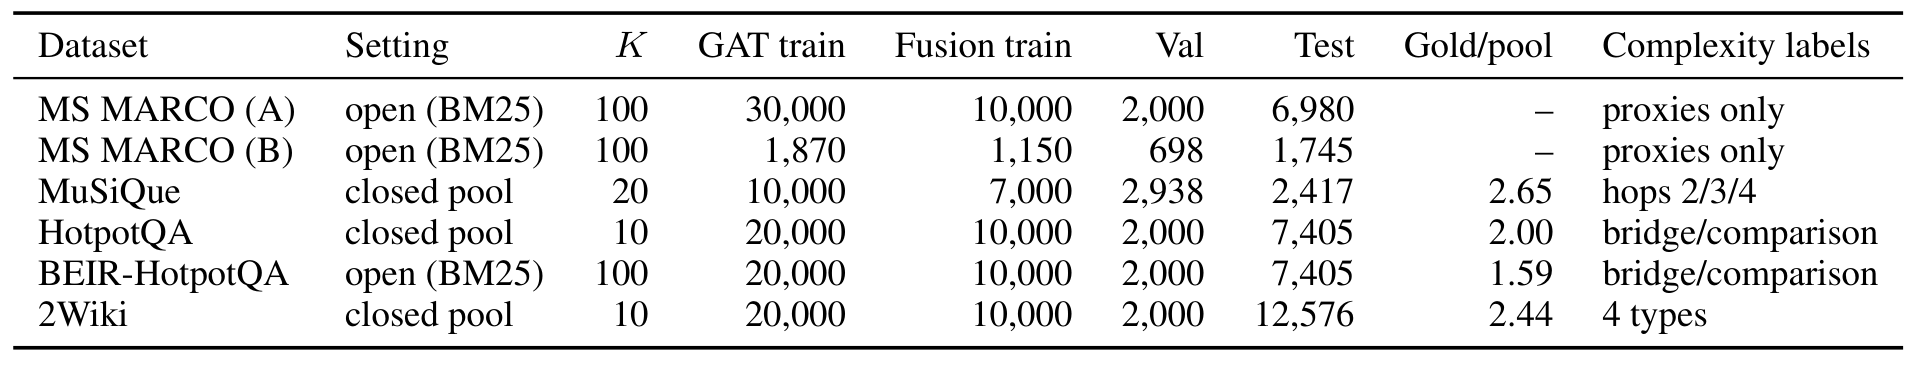
\includegraphics[width=0.85\textwidth]{img/table1.png}
\src{Table 1 of our report. Open: BM25 pool from the full corpus. Closed: the dataset's own paragraphs.}
\end{frame}

% ================================================================ results
\divider{Part 3}{Results}

\begin{frame}{1.\ The best $\alpha$ differs by dataset}
\centering
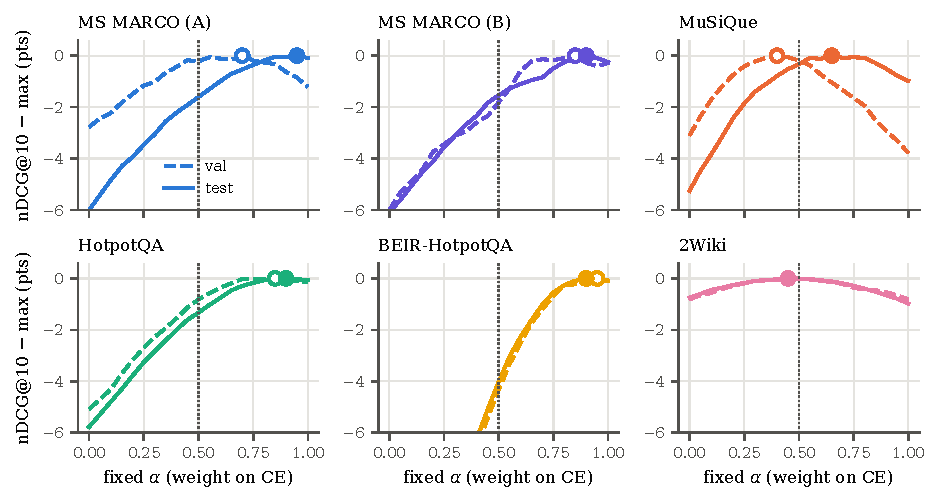
\includegraphics[height=0.66\textheight]{img/alpha_curves.pdf}\\[0.1cm]
\begin{minipage}{0.92\textwidth}\small
nDCG@10 vs.\ fixed $\alpha$. MS MARCO peaks at a high $\alpha$ (\textbf{0.70--0.95}); the multi-hop sets MuSiQue (val \textbf{0.40}) and 2Wiki (\textbf{0.45}) peak \hl{below 0.5}.
\end{minipage}
\src{Figure 1 of our report (min--max, dashed = val, solid = test).}
\end{frame}

\begin{frame}{1.\ More hops $\Rightarrow$ lower $\alpha$ (MuSiQue)}
\centering
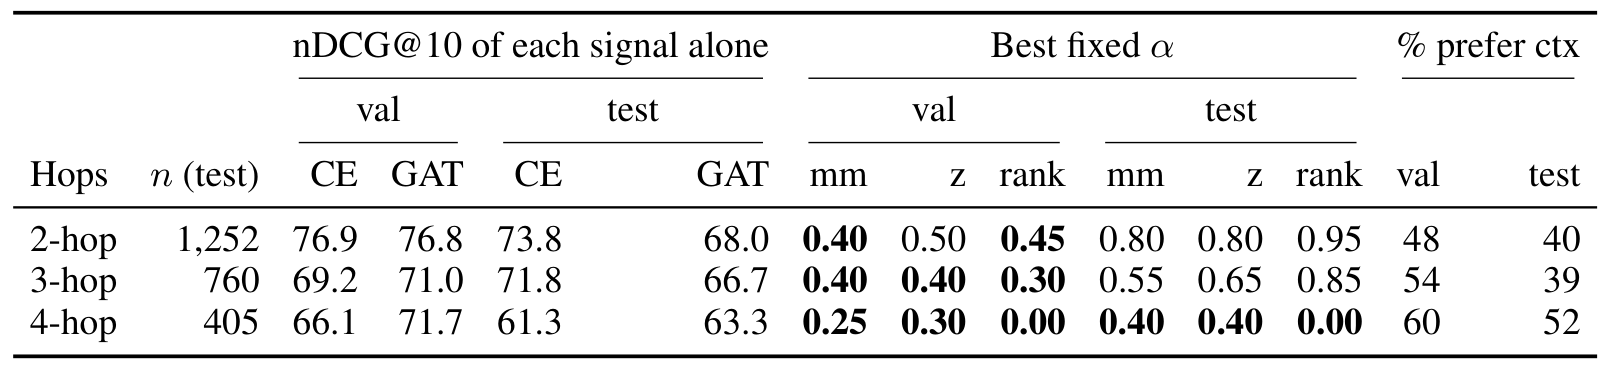
\includegraphics[width=0.94\textwidth]{img/table3.png}\\[0.4cm]
\begin{columns}[T]
\begin{column}{0.46\textwidth}
\cardbox[ctxcard]{6.1cm}{\small\textbf{Best $\alpha$ falls with each hop} under every normaliser. Test, min--max: \textbf{0.80 $\to$ 0.55 $\to$ 0.40}; val: 0.40 $\to$ 0.40 $\to$ 0.25.}
\end{column}
\begin{column}{0.46\textwidth}
\cardbox[semcard]{6.1cm}{\small\textbf{Why:} from 2 to 4 hops the cross-encoder drops 12.5 nDCG points (test), the GAT only 4.7. At 4 hops the GAT is ahead.}
\end{column}
\end{columns}
\src{Table 3 of our report. mm = min--max, z = z-score.}
\end{frame}

\begin{frame}{1.\ The trend holds under every normaliser}
\begin{columns}[c]
\begin{column}{0.5\textwidth}
\centering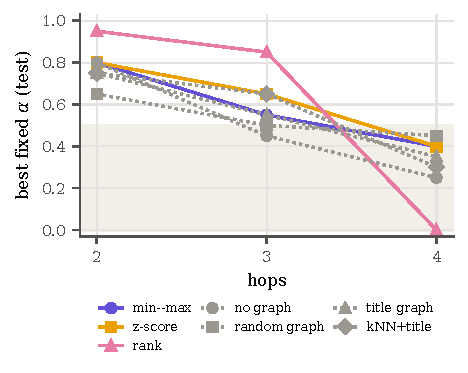
\includegraphics[width=\linewidth]{img/hops_robust.pdf}
\src{Figure 3 of our report (MuSiQue test).}
\end{column}
\begin{column}{0.46\textwidth}
\begin{itemize}\setlength{\itemsep}{8pt}
  \item Min--max, z-score and rank all give a \hl{monotone decline} of the best $\alpha$ from 2 to 4 hops.
  \item 4-hop questions sit \textbf{below 0.5} in all 14 normaliser / graph / split settings.
  \item Per question: preferred $\alpha$ correlates negatively with hop count (Spearman $\rho\approx-0.07$, $p\le0.004$ on val and test).
\end{itemize}
\end{column}
\end{columns}
\end{frame}

\begin{frame}{1.\ Same pattern by question type (2Wiki)}
\centering
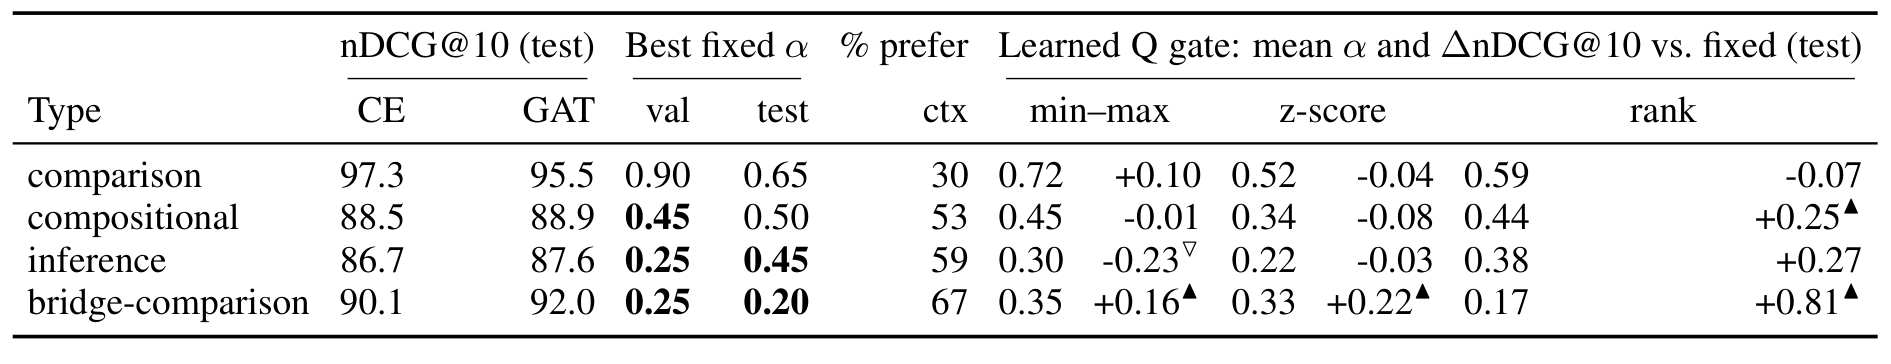
\includegraphics[width=0.96\textwidth]{img/table4.png}\\[0.4cm]
\begin{columns}[T]
\begin{column}{0.3\textwidth}
\cardbox[semcard]{3.9cm}{\small\textbf{Comparison}:\\$\alpha=0.65$--$0.90$,\\cross-encoder wins.}
\end{column}
\begin{column}{0.3\textwidth}
\cardbox[ctxcard]{3.9cm}{\small\textbf{Inference, bridge-comp.}:\\$\alpha=0.20$--$0.45$,\\GAT wins.}
\end{column}
\begin{column}{0.33\textwidth}
\cardbox[card]{4.3cm}{\small\textbf{Q gate}, blind to the type: highest $\alpha$ on comparison, gains on bridge-comp.}
\end{column}
\end{columns}
\src{Table 4 of our report. Bold: $\alpha<0.5$. $\blacktriangle$: significantly better than fixed $\alpha$ ($p<0.05$).}
\end{frame}

\begin{frame}{2.\ Adaptive $\alpha$ gains on complex queries}
\begin{columns}[c]
\begin{column}{0.58\textwidth}
\centering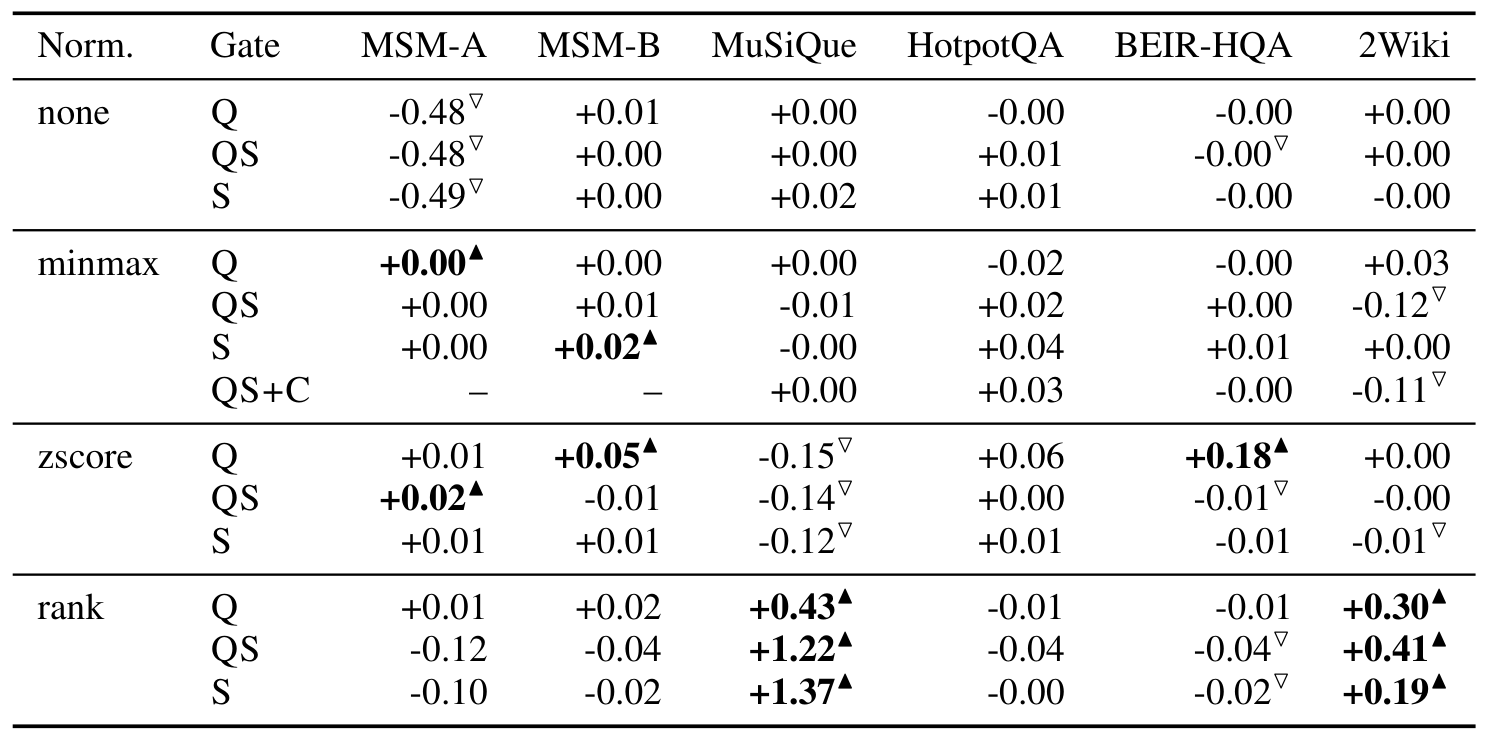
\includegraphics[width=\linewidth]{img/table6.png}
\src{Table 6 of our report: $\Delta$nDCG@10 vs.\ best fixed $\alpha$ (test).}
\end{column}
\begin{column}{0.39\textwidth}
\begin{itemize}\setlength{\itemsep}{6pt}\small
  \item \textbf{7 of the 11} significant gains are on the \hl{multi-hop} sets.
  \item Largest: MuSiQue, rank norm., \textbf{+0.43 / +1.22 / +1.37} (Q / QS / S).
  \item MS MARCO gains $\le 0.05$: one fixed $\alpha$ serves simple queries.
  \item Oracle per-query $\alpha$ headroom: 7.4 (MuSiQue) vs.\ 5.0 (MS MARCO).
\end{itemize}
\end{column}
\end{columns}
\end{frame}

\begin{frame}{2.\ Transfer: $\alpha$ follows the target data}
\centering
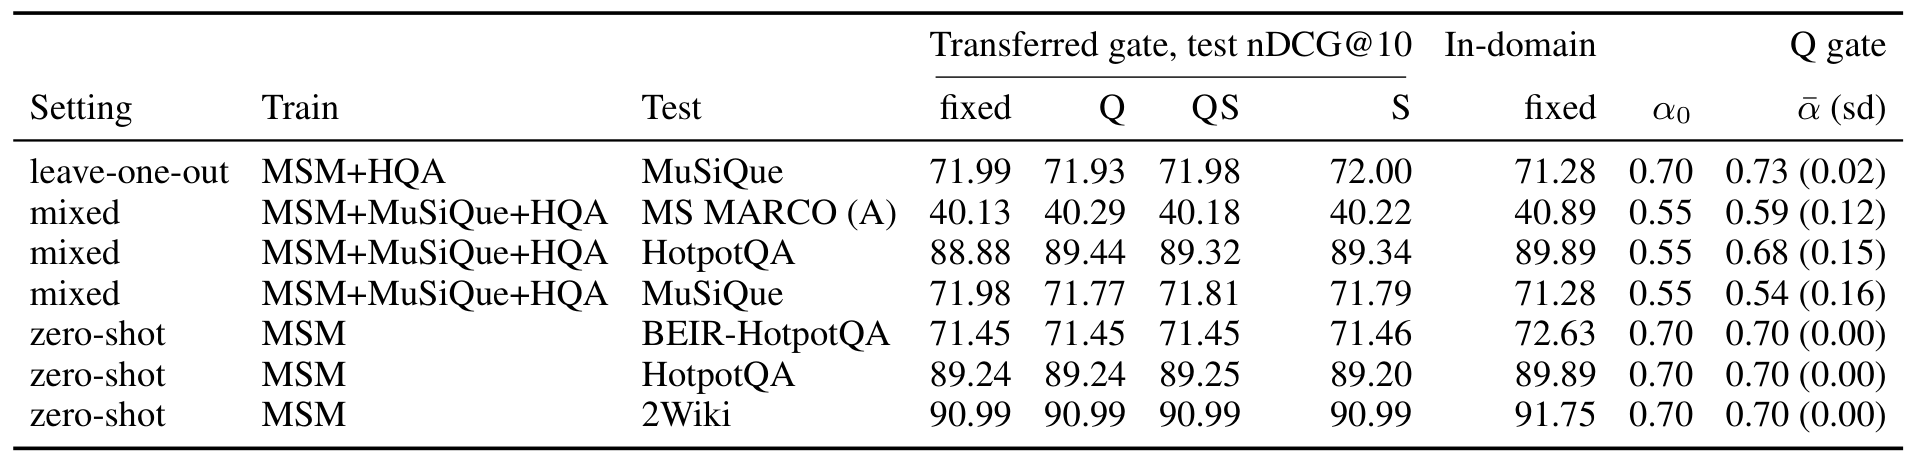
\includegraphics[width=0.94\textwidth]{img/table9.png}\\[0.35cm]
\begin{columns}[T]
\begin{column}{0.46\textwidth}
\cardbox[ctxcard]{6.1cm}{\small\textbf{One gate on mixed data} (MS MARCO + MuSiQue + HotpotQA) gives MuSiQue the \textbf{lowest} mean $\alpha$ (0.54) vs.\ MS MARCO 0.59 and HotpotQA 0.68.}
\end{column}
\begin{column}{0.46\textwidth}
\cardbox[semcard]{6.1cm}{\small\textbf{Zero-shot} MS MARCO gates keep $\alpha=0.70$ and lose to the target's own setting, e.g.\ 2Wiki 90.99 vs.\ 91.75 (in-domain $\alpha_0=0.45$).}
\end{column}
\end{columns}
\src{Table 9 of our report (min--max, test nDCG@10 $\times100$, 5 seeds).}
\end{frame}

\begin{frame}{Conclusion}
\begin{columns}[T]
\begin{column}{0.56\textwidth}
\begin{itemize}\setlength{\itemsep}{7pt}\small
  \item \textbf{Alpha follows the hops}: the more reasoning steps a query needs, the more weight belongs on the graph-contextual score.
  \item MuSiQue: best $\alpha$ 0.80 $\to$ 0.55 $\to$ 0.40 for 2 $\to$ 3 $\to$ 4 hops; 4-hop below 0.5 in every setting.
  \item Mechanism: the cross-encoder degrades with hops much faster than the GAT.
  \item One fixed weight is a compromise; query-dependent gates gain mostly on multi-hop data.
\end{itemize}
\end{column}
\begin{column}{0.4\textwidth}
\cardbox[card]{5.3cm}{\textbf{Limits}\\[0.1cm]\small
HotpotQA keeps a high $\alpha$ (single-hop shortcuts). Min--max gates mostly stay at their start value.}
\vspace{0.3cm}

\cardbox[ctxcard]{5.3cm}{\textbf{Next}\\[0.1cm]\small
Gates with explicit complexity signals (predicted hop count), and fusing at the passage-pair level.}
\end{column}
\end{columns}
\end{frame}

{\setbeamercolor{background canvas}{bg=ink}\setbeamertemplate{footline}{}
\begin{frame}[plain]
  \vfill\begin{center}{\color{white}\fontsize{36}{40}\selectfont\bfseries Thank you}\\[0.4cm]
  {\color{ctx}\Large Questions?}\end{center}\vfill
  {\color{white!70!ink}\scriptsize
  MacAvaney, Tonellotto, Macdonald. Adaptive Re-Ranking with a Corpus Graph. CIKM 2022.\\
  Brody, Alon, Yahav. How Attentive are Graph Attention Networks? ICLR 2022.\quad
  Trivedi et al. MuSiQue. TACL 2022.\\
  Yang et al. HotpotQA. EMNLP 2018.\quad Ho et al. 2WikiMultiHopQA. COLING 2020.\quad
  Nguyen et al. MS MARCO. 2016.\quad Thakur et al. BEIR. NeurIPS 2021.}
\end{frame}}

\end{document}
